\section{The Wu Experiment \cite{wu}}
The Wu experiment was the first experiment that proved a maximum parity violation in the weak $\beta$ decay. It was the first confirmation towards the chiral nature of the weak interaction.
\subsection{Historical Context}
The parity $\hat{P}$ operator transforms a phenomen into its mirror image. A phenomen that is not identical to its mirror image is called chiral. Measurements of electromagnetic and strong interaction showed invariance under parity. As a result it was accepted that the mirror image of any physical process shows the same physics. In 1956 physicists believed that a system is invariant under the combination ($CPT$ theorem) of parity $\hat{P}$, charge conjugation $\hat{C}$ and time reversal $\hat{T}$ as well as under each operation itself. In 1953 R.H. Dalitz adressed the so called $\tau-\theta$-puzzle which decribes the decay of two charged strange mesons:
\begin{align*}
  \tau^+ &= \pi^+ \pi^+ \pi^- & \hat{P}\ket{\tau} = -1 \ket{\tau}\\
  \theta^+ &= \pi^+ \pi^0 & \hat{P}\ket{\theta} = +1 \ket{\theta}
\end{align*}
Both particles have the same spin, charge, mass and lifetime, but different parity eigenvalues. Due to the principle of parity conservation this indicates that these are still to different particles. 1956 Lee and Yang proposed that $\tau$ and $\theta$ could be the same particle if the weak interaction violates parity conservation. They reviewed previous measurements and could not find any that ruled out the possibility of a chiral weak interaction. Hence they proposed that experimental states are a misture of states with usual and opposite parity. This leads to coupling constants $C$ for parity conserving and $C^{'}$ for nonconserving interactions as well as $CC^{'}$ interference terms. It was not possible to distinguish between $C$ and $C^{'}$ since the neutrino spin was not known back at the time. The misture has an effect on the angular distribution of nuclear interactions:
\begin{align*}
	I(\vartheta) \text{d}\vartheta \propto (1 + \alpha \cos \vartheta) \sin\vartheta \text{d}\theta
\end{align*}
where $\alpha$ is the asymmetry coefficient that contains the interference terms with $CC^{'}$. Lee and Yang proposed numerous possibilities to study the parity conservation of the weak interaction e.g. the angular distribution between an electron and a nucleus of a $\beta$ decay.

\subsection{Experimental Setup}
% \begin{wrapfigure}{l}{0.31\textwidth}
%     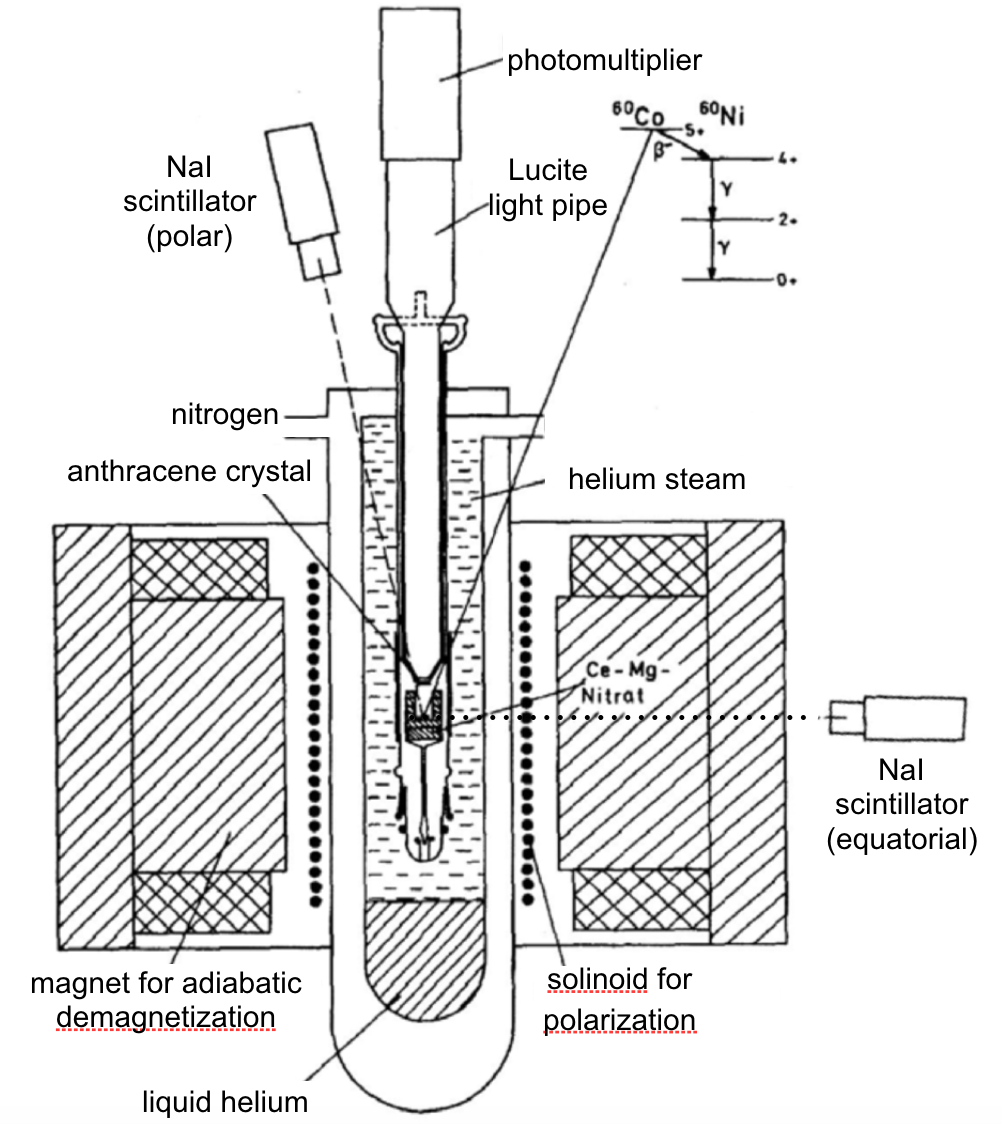
\includegraphics[width=0.3\textwidth]{graphics/Wu_setup.png}
%     \caption{Experimental setup of the Wu experiment. \cite{wu}}
% 		\label{fig:Wu_setup}
%   \end{wrapfigure}
%   \FloatBarrier
The Wu experiment was carried out at the National Bureau of Standards (NBS) in Washington, D.C., by Chien-Shieung Wu and her low temperature group in 1956.
They used the suggested $\beta$ decay of a nucleus to verify if the weak interaction is chiral or not. The underlying principle was that changing the direction of the nucleus polarization is equivalent to a parity transformation. \\
One of the main challenges was the selection of the right nucleus for the experiment. They used $^{60}Co$ nuclei, because the corresponding $\beta$ decay is a Gamow-Telller transition, where the emitted particles have a parallel spin. This is necessary to determine the chiral nature of the weak interaction.
\begin{align*}
  ^{60}Co &\rightarrow \ ^{60}Ni^{*} + e^- + \bar{\nu}_e \label{eqn:kobalt-zerfall}\\
  ^{60}Ni^{*} & \rightarrow \ ^{60}Ni + 2 \, \gamma \\
\end{align*}
The second benefit is that the photons are emitted in the direction of the nucleus polarization. Therefore measuring the emitted photons allows to determine the polarization degree of the $^{60}Co$ nuclei. Two NaI scintillator are placed in a polar and equatorial position to the specimen to measure the photons. The specimen is placed inside of a cryostat with a anthracene crystal at the top end to detected the $\beta$ particles and emit photons which are then counted with a photomultiplier at the end of a Lucite light pipe. The photomultiplier is sensitiv to a specific energy corresponding to the energy of the $\beta$ particle.
Since the magnet moment of the electron is much greater as the one of the nucleus, a temperature close to absolute zero is necessary to polarize the nucleus. This method is called Gorter-Rose method and uses the principle of adaibatic demagnetization. The applied magnetic field reduces the entropy of the magnetic moments, afterwards the specimen is isolated adiabaticly and the magnet switched off. The present entropy of the system corresponds to a much lower temperature, which leads to instant cooling of the specimen. The used cerium magnesium nitrate bas a high anisotropic Landé g-factor ($g_1 \ll g_2$). This allows to apply a high magnetic field along $g_1$ with the first magnet and cool the salt down to around $\SI{0.003}{\kelvin}$. Afterwards a solinoid is used to polarize the salt in direction of the second g-factor. The polarization of the orbital electrons enhance the magnetic field close to the nucleus. To use this effect a thin layer of $^{60}Co$ is vaporised on a CeMg nitrate crystal which together builds the specimen.
\subsection{Results}
\begin{wrapfigure}{l}{0.4\textwidth}
    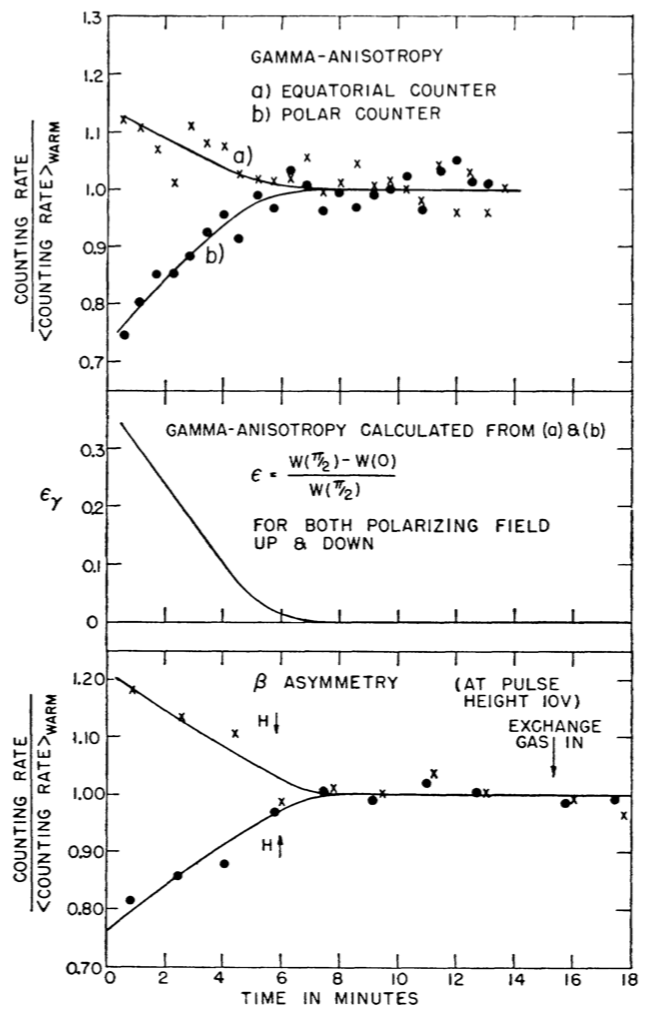
\includegraphics[width=0.35\textwidth]{graphics/Wu_result.png}
    \caption{Gamma anisotropy and beta asymmetry for polarizing field pointing in positive and negative $z$ direction. \cite{wu}}
		\label{fig:Wu_result}
  \end{wrapfigure}
  \FloatBarrier
The spins of the neutrinos and electrons point in the same direction as the spin of the mother core due angular momentum conservation.
Due to the polarization of the nuclei the spin direction is parallel to the magnetic field.
Reversing the polarization of the magnetic field is identical to a parity transformation. The quantity of the emitted electrons was measured in negative $z$ direction for both polarizations of the magnetic field. If parity is conserved the same amount of electrons will be emitted parallel and antiparallel to the nucleus spin. Therefore the same amount of electrons should be measured for both magnetic field configurations.\\
The top and the bottom diagram in figure \ref{fig:Wu_result} are normalized with the counting rate of the warm setup, when the nuclei are not polarized. The top diagram shows the gamma anisotropy for the equatorial and the polar counter. It clearly shows that the polar counter is count less events compared to the warm configuration. From this rates are used to calculate the gamma anisotropy that is shown in the middle diagram. At the beginning a anisotropy of around \SI{40}{\percent} is seen, which corresponds to a polarization  degree of \SI{60}{\percent} for the cobald nuclei. After around \SI{6}{\minute} the setup is back to the unpolarized configuration. The bottom diagram final shows the $\beta$ asymmetry for both magnetic field configuration. For the downwards direction the counting rate is exactly the same amount higher than the amount missing for the upward field direction. Furthermore the curse of the data point fits exactly the curse of the gamma anisotropy. This leads to the conclusion that the parity conservation is not only violated, but at a maximum.\\
Around the same time the Columbia experiment studied the angular destribution of a pion beam decaying weakly into muons, which then decay into electrons. They carried it out under the assumption that the muon is highly polarized if parity conservation is violated. They used a solinoid to change the orientation of the polarized muons and observed as well a large asymmetry corresponding to the changing field. Which shows again that parity conservation is violated.
